\chapter{Hormonale regeling van de voortplanting}\label{ch:b2:reproductive-hormones}

Elke maand, dertig jaar lang volgens een schema dat tot op een of twee
dagen nauwkeurig is, rijpt er één \omterm{def:b2:mammal-reproduction:ovary}{follikel}, komt er één eicel vrij, wordt
het slijmvlies van de baarmoeder opgebouwd en daarna, tenzij er een embryo
is aangekomen, weer afgebroken. Geen enkele klok in het lichaam tikt in dit
tempo; het ritme ontstaat uit een gesprek tussen drie organen --- de
hypothalamus, de hypofyse en het ovarium --- waarin elk hormoon de afgifte
van het volgende regelt en het laatste het eerste regelt. Dit hoofdstuk
ontleedt dat gesprek: de as die beide geslachten stuurt, de tonische
regeling van de \omterm{def:b2:mammal-reproduction:testis}{testis}, de cyclische regeling van het ovarium met zijn
opmerkelijke omslag van negatieve naar positieve terugkoppeling, en de
manieren waarop de as wordt overstemd door zwangerschap, door
geneesmiddelen en door de kliniek.

\section{De as}

\begin{definition}[De hypothalamus-hypofyse-gonade-as]\label{def:b2:reproductive-hormones:axis}
\index{gonadotrofine-releasing hormoon}\index{luteïniserend hormoon}\index{follikelstimulerend hormoon}\index{negatieve terugkoppeling!hormonale}
Neuronen van de \emph{hypothalamus} scheiden \emph{GnRH}
(gonadotrofine-releasing hormoon, een peptide van tien aminozuren) af in
de kleine poortvaten die naar de \emph{voorkwab van de hypofyse} lopen,
in korte \emph{pulsen} om de een tot twee uur. GnRH laat de hypofyse twee
glycoproteïnehormonen afscheiden in de algemene circulatie, de
\emph{gonadotrofinen} \emph{LH} (luteïniserend hormoon) en \emph{FSH}
(follikelstimulerend hormoon). Deze werken in op de \emph{gonaden}: LH op
de steroïdproducerende cellen (leydigcellen, theca- en luteale cellen), FSH
op de cellen die de gameten verzorgen (sertoli- en granulosacellen). De
gonaden antwoorden met steroïden ---
\emph{testosteron}, \emph{oestradiol}, \emph{progesteron} --- en met het
peptide \emph{inhibine}, en die koppelen terug op hypothalamus en hypofyse:
de steroïden op beide, meestal \emph{negatief}; inhibine alleen op FSH. Het
resultaat is een geregelde lus waarin de productie van de gonade op een
instelwaarde wordt gehouden, en hetzelfde ontwerp met drie niveaus stuurt de
schildklier en de bijnierschors. De mechanismen waarmee deze hormonen op hun
cellen inwerken, zijn het onderwerp van \cref{ch:b2:cell-signalling}.
\end{definition}

\begin{omfigure}
\begin{tikzpicture}[every node/.style={font=\scriptsize}, >=stealth]
  \node[draw, rounded corners, fill=omDef!15, align=center, minimum width=3cm] (hyp) at (0,4.2) {hypothalamus\\GnRH, in pulsen};
  \node[draw, rounded corners, fill=omDef!15, align=center, minimum width=3cm] (pit) at (0,2.2) {hypofysevoorkwab\\LH en FSH};
  \node[draw, rounded corners, fill=omProp!20, align=center, minimum width=3cm] (gon) at (0,0) {gonade\\steroïden, inhibine};
  \node[draw, rounded corners, fill=omExo!25, align=center, minimum width=3cm] (tar) at (5.2,0) {doelweefsels\\gametogenese, gangen,\\secundaire kenmerken};
  \draw[->, thick] (hyp) -- (pit) node[midway, right] {poortvaten};
  \draw[->, thick] (pit) -- (gon) node[midway, right] {bloed};
  \draw[->, thick] (gon) -- (tar);
  \draw[->, thick, omThm] (gon.west) .. controls (-3.0,0) and (-3.0,2.2) .. (pit.west);
  \draw[->, thick, omThm] (gon.west) .. controls (-4.6,0) and (-4.6,4.2) .. (hyp.west);
  \node[omThm, anchor=east, align=right] at (-3.9,1.2) {naar de hypofyse:\\steroïden $(-)$,\\inhibine $(-)$ op FSH};
  \node[omThm, anchor=east, align=right] at (-3.9,3.6) {naar de hypothalamus:\\steroïden $(-)$\\(oestradiol $(+)$\\halverwege de cyclus)};
\end{tikzpicture}

{\small De as: GnRH uit de hypothalamus stuurt LH en FSH uit de hypofyse
aan, die de gonade aansturen; de steroïden en de inhibine van de gonade
koppelen negatief terug op beide hogere niveaus --- behalve de korte
positieve terugkoppeling van oestradiol die de \omterm{def:b2:mammal-reproduction:ovary}{ovulatie} in gang zet.}
\end{omfigure}

\begin{proposition}[Waarom de pulsen ertoe doen]\label{prop:b2:reproductive-hormones:pulses}
\index{pulsatiele secretie}\index{desensitisatie van receptoren}
De hypofyse reageert alleen op GnRH als het in pulsen aankomt. Een cel die
voortdurend aan een hormoon wordt blootgesteld, haalt de receptoren van
dat hormoon van haar oppervlak (\emph{desensitisatie}); als de
receptorvoorraad wordt aangevuld met een snelheid $s$, verwijderd met een
basale snelheid $d$ en, in aanwezigheid van hormoon $H$, met een extra
snelheid $iH$, dan geldt
\[
\frac{\mathrm{d}R}{\mathrm{d}t} = s - (d + iH)\,R, \qquad R^* = \frac{s}{d + iH},
\]
zodat een voortdurend hoge $H$ het aantal receptoren naar een lage
stationaire toestand drijft en de cel stilvalt, terwijl korte pulsen,
gescheiden door hormoonvrije intervallen, de voorraad ertussen laten
herstellen (tijdconstante $1/d$). Een GnRH-puls om de negentig
minuten houdt de hypofyse gevoelig; een constant infuus, of een langwerkende
GnRH-agonist, legt haar binnen enkele dagen stil --- de grondslag van de
geneesmiddelen die de as onderdrukken bij prostaatkanker, endometriose en
vroegtijdige puberteit. De pulsfrequentie codeert ook informatie:
snelle pulsen bevoordelen LH, trage pulsen FSH.
\end{proposition}
\begin{proof}[Bewijsmateriaal]
Knobil (1978--1980) vernietigde de GnRH-neuronen van resusapen, wat LH,
FSH en de cyclus deed verdwijnen, en verving GnRH vervolgens door een
pomp: één puls per uur herstelde de gonadotrofinen en normale
ovulatoire cycli; dezelfde dagdosis, continu toegediend, herstelde ze
enkele dagen en daarna zakten LH en FSH in tot nul; terugkeren naar
pulsen herstelde ze opnieuw. Het toedieningspatroon, niet de hoeveelheid,
is het signaal.
\end{proof}

\begin{omfigure}
\begin{tikzpicture}
\begin{axis}[
  width=0.8\linewidth, height=5.4cm,
  axis x line=bottom, axis y line=left,
  xmin=0, xmax=40, ymin=0, ymax=1.2,
  xlabel={dagen}, ylabel={LH in plasma (relatief)},
  xlabel style={font=\small, at={(axis description cs:0.5,-0.13)}, anchor=north},
  ylabel style={font=\small},
  tick label style={font=\small}, xtick={0,10,20,30,40}, ytick={0,0.5,1},
  clip=false,
]
\addplot[very thick, omDef, domain=0:10, samples=2] {1};
\addplot[very thick, omThm, domain=10:25, samples=60] {exp(-(x-10)/3)};
\addplot[very thick, omDef, domain=25:40, samples=60] {1-exp(-(x-25)/2)};
\fill[omDef!15] (axis cs:0,1.05) rectangle (axis cs:10,1.15); \node[font=\scriptsize] at (axis cs:5,1.1) {pulsen per uur};
\fill[omThm!15] (axis cs:10,1.05) rectangle (axis cs:25,1.15); \node[font=\scriptsize] at (axis cs:17.5,1.1) {continu infuus};
\fill[omDef!15] (axis cs:25,1.05) rectangle (axis cs:40,1.15); \node[font=\scriptsize] at (axis cs:32.5,1.1) {weer pulsen};
\end{axis}
\end{tikzpicture}

{\small Het experiment van Knobil, schematisch. Bij een aap van wie de eigen
GnRH-neuronen zijn vernietigd, houden pulsen GnRH om het uur LH in stand;
overschakelen op een continu infuus van dezelfde dagelijkse hoeveelheid
dooft het binnen enkele dagen uit, en pulsen herstellen het.}
\end{omfigure}

\begin{omfigure}
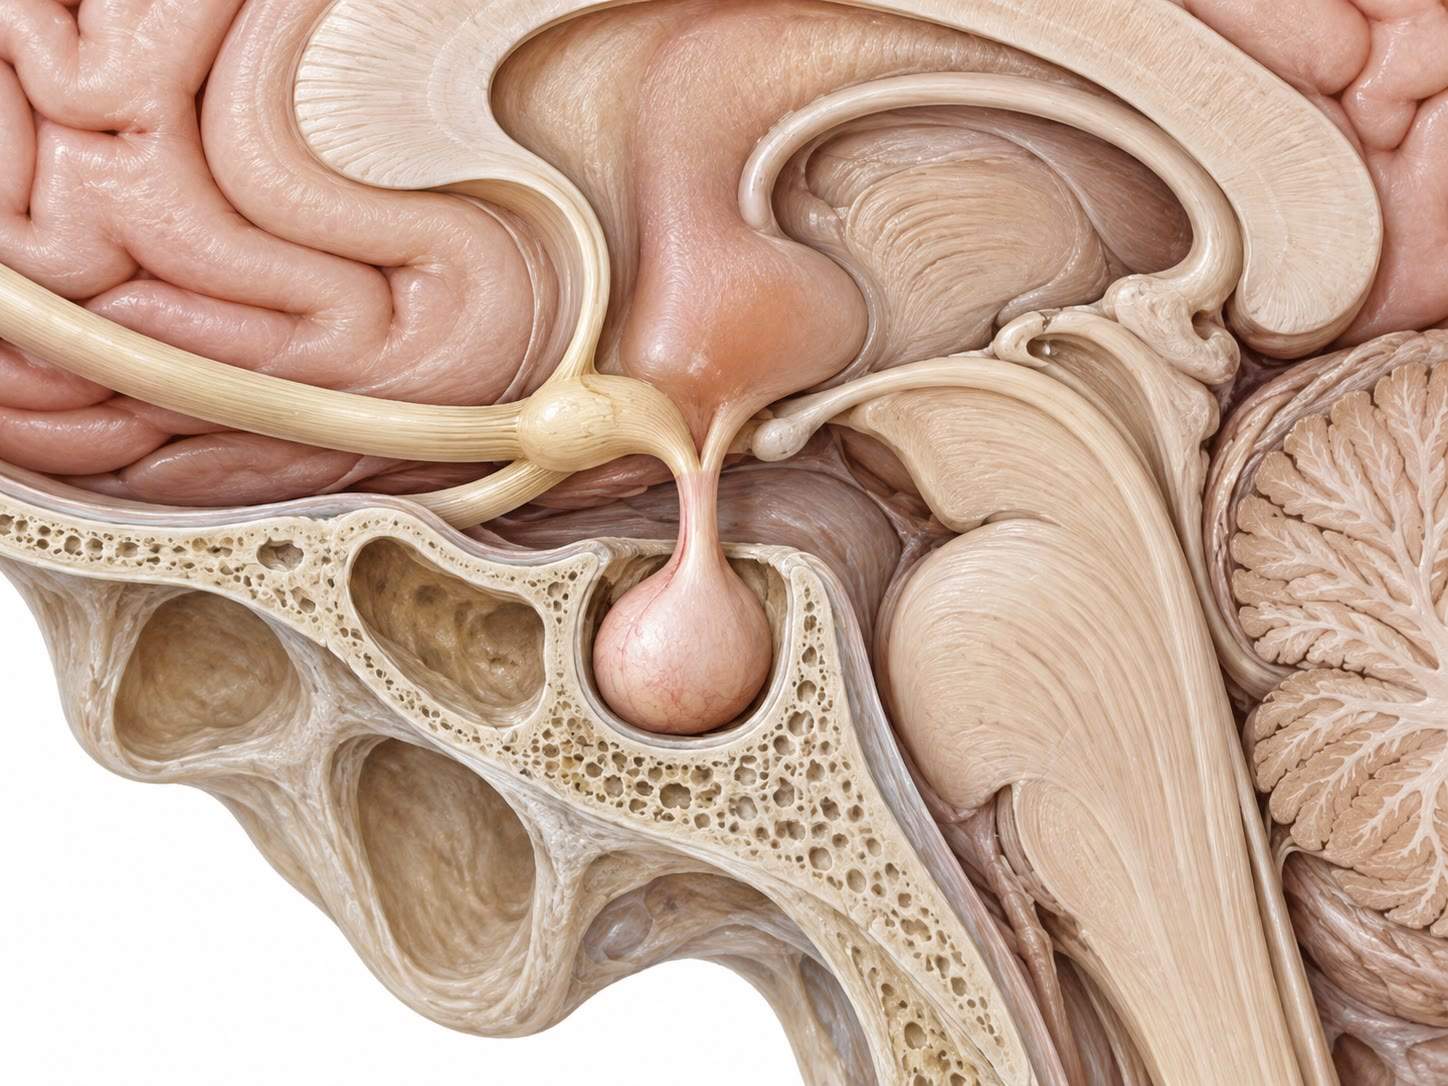
\includegraphics[width=0.55\linewidth]{images/book4/ai/b4-09-hypothalamus-pituitary.jpg}

{\small De hersenbasis in sagittale doorsnede: de hypothalamus erboven, de
steel, en de hypofyse in haar benige holte --- de hardware van de as.}
\end{omfigure}

\section{De man: tonische regeling}

\begin{proposition}[Regeling van de testis]\label{prop:b2:reproductive-hormones:testis}
\index{testosteron}\index{inhibine}
LH werkt in op de leydigcellen, die \emph{testosteron} maken
(\qtyrange{3}{10}{ng/mL} in het bloed van een volwassen man, honderd keer
meer in de \omterm{def:b2:mammal-reproduction:testis}{testis} zelf). FSH werkt in op de sertolicellen, die --- samen met
het lokale testosteron --- de \omterm{def:b2:mammal-reproduction:testis}{spermatogenese} ondersteunen en
\emph{inhibine} afscheiden. Testosteron koppelt terug op hypothalamus en
hypofyse om LH laag te houden; inhibine koppelt terug op de hypofyse om FSH
laag te houden. Beide lussen zijn \emph{negatief} en het systeem is
\emph{tonisch}: de hormoonspiegels schommelen met de pulsen en met het
tijdstip van de dag (het hoogst 's ochtends), maar vertonen geen cyclus, en
zaadcellen worden continu gemaakt. Testosteron bouwt en onderhoudt ook de
accessoire klieren en gangen, de baard, de stem, spieren en botten, de
aanmaak van rode bloedcellen en het libido, en maakte bij de foetus het
mannelijke lichaam (\cref{ch:b2:mammal-reproduction}). Castratie neemt het
weg: LH en FSH stijgen bij gebrek aan terugkoppeling tot een veelvoud, en de
secundaire kenmerken gaan in regressie; ingespoten testosteron herstelt de
kenmerken --- maar niet de vruchtbaarheid, omdat het ook LH onderdrukt en
daarmee het testosteron in de \omterm{def:b2:mammal-reproduction:testis}{testis} dat de \omterm{def:b2:mammal-reproduction:testis}{spermatogenese} nodig heeft.
Daarom maken anabole steroïden mannen onvruchtbaar.
\end{proposition}
\begin{proof}[Bewijsmateriaal]
Berthold (1849) castreerde jonge hanen: hun kammen kromp in en ze kraaiden
noch vochten. Een \omterm{def:b2:mammal-reproduction:testis}{testis} die in de buikholte van een gecastreerde haan werd
getransplanteerd, waar hij een nieuwe bloedvoorziening kreeg maar geen
zenuwen, herstelde kam, gekraai en vechtlust: de \omterm{def:b2:mammal-reproduction:testis}{testis} werkte via het
bloed --- het eerste bewijs van een inwendige secretie, vijftig jaar vóór
het woord hormoon. Testosteron werd in 1935 geïsoleerd en gesynthetiseerd.
\end{proof}

\section{De vrouw: een cyclus met een schakelaar}

\begin{definition}[De ovariële en de uteriene cyclus]\label{def:b2:reproductive-hormones:cycle}
\index{menstruatiecyclus}\index{folliculaire fase}\index{luteale fase}\index{LH-piek}\index{endometrium}
De cyclus wordt geteld vanaf de eerste dag van de menstruatie en duurt
ongeveer 28 dagen. \emph{Folliculaire fase} (dag 1--14): FSH, door de dood
van het vorige \omterm{def:b2:mammal-reproduction:ovary}{corpus luteum} van terugkoppeling bevrijd, rekruteert een
cohort \omterm{def:b2:mammal-reproduction:ovary}{follikels}; die scheiden \emph{oestradiol} af, dat gestaag stijgt;
oestradiol en inhibine verlagen FSH, en alleen de \omterm{def:b2:mammal-reproduction:ovary}{follikel} met de meeste
FSH-receptoren overleeft die daling --- de dominante \omterm{def:b2:mammal-reproduction:ovary}{follikel}. In de
baarmoeder bouwt oestradiol het \emph{endometrium} weer op (de
proliferatieve fase) en maakt het het slijm van de baarmoederhals dunner.
\emph{\omterm{def:b2:mammal-reproduction:ovary}{Ovulatie}} (dag 14): wanneer oestradiol anderhalve dag boven ongeveer
\qty{200}{pg/mL} is gebleven, slaat zijn terugkoppeling op hypothalamus en
hypofyse om van negatief naar \emph{positief}; LH stijgt in een dag
tienvoudig --- de \emph{LH-piek} --- en ongeveer 36 uur na het begin ervan
barst de \omterm{def:b2:mammal-reproduction:ovary}{follikel} open en laat de oöcyt vrij. \emph{Luteale fase} (dag
15--28): de lege \omterm{def:b2:mammal-reproduction:ovary}{follikel} wordt het \omterm{def:b2:mammal-reproduction:ovary}{corpus luteum}, dat onder invloed van LH
\emph{progesteron} (\qtyrange{10}{20}{ng/mL}) en oestradiol afscheidt;
progesteron maakt het endometrium secretorisch, maakt het slijm dikker,
verhoogt de basale lichaamstemperatuur met \qty{0.3}{\celsius}, en
onderdrukt samen met oestradiol LH en FSH. Het \omterm{def:b2:mammal-reproduction:ovary}{corpus luteum} heeft een
levensduur van ongeveer 14 dagen; tenzij hCG van een embryo het redt, gaat
het in regressie, dalen progesteron en oestradiol, wordt het endometrium
afgestoten (\emph{menstruatie}), stijgt FSH, en begint de volgende cyclus.
De luteale fase ligt vast op 14 dagen; variatie in de cyclusduur is
variatie in de folliculaire fase.
\end{definition}

\begin{omfigure}
\begin{tikzpicture}
\begin{axis}[
  width=0.94\linewidth, height=6.4cm,
  axis x line=bottom, axis y line=left,
  xmin=0, xmax=28, ymin=0, ymax=1.15,
  xlabel={dag van de cyclus}, ylabel={hormonen (relatief t.o.v.\ piek)},
  xlabel style={font=\small, at={(axis description cs:0.5,-0.11)}, anchor=north},
  ylabel style={font=\small},
  tick label style={font=\small}, xtick={0,7,14,21,28}, ytick={0,0.5,1},
  legend style={font=\scriptsize, at={(0.5,-0.25)}, anchor=north, draw=none, legend columns=4},
  clip=false,
]
\addplot[very thick, omThm, domain=0:28, samples=120] {0.1 + 0.9*exp(-((x-14)^2)/0.9)};
\addlegendentry{LH}
\addplot[very thick, omProp, domain=0:28, samples=120] {0.35*exp(-x/6) + 0.15 + 0.35*exp(-((x-14)^2)/1.2)};
\addlegendentry{FSH}
\addplot[very thick, omDef, domain=0:28, samples=160] {0.1 + 0.9*exp(-((x-12.5)^2)/6) + 0.4*exp(-((x-21)^2)/12)};
\addlegendentry{oestradiol}
\addplot[very thick, omExo!70!black, domain=0:28, samples=160] {0.03 + 0.97*exp(-((x-21)^2)/12)*(x>14)};
\addlegendentry{progesteron}
\draw[dashed, gray] (axis cs:14.5,0) -- (axis cs:14.5,1.1); \node[font=\scriptsize, anchor=south] at (axis cs:14.5,1.1) {ovulatie};
\node[font=\scriptsize, anchor=north] at (axis cs:7,1.1) {folliculaire fase};
\node[font=\scriptsize, anchor=north] at (axis cs:21.5,1.1) {luteale fase};
\end{axis}
\end{tikzpicture}

{\small De hormonen van de cyclus. Oestradiol uit de groeiende \omterm{def:b2:mammal-reproduction:ovary}{follikel}
stijgt tijdens de \omterm{def:b2:reproductive-hormones:cycle}{folliculaire fase} en zet, voorbij een drempel, de
\omterm{def:b2:reproductive-hormones:cycle}{LH-piek} in gang; de \omterm{def:b2:mammal-reproduction:ovary}{ovulatie} volgt ongeveer 36 uur later; het \omterm{def:b2:mammal-reproduction:ovary}{corpus
luteum} scheidt daarna twee weken progesteron af en sterft.}
\end{omfigure}

\begin{omfigure}
\begin{tikzpicture}[every node/.style={font=\scriptsize}]
  % endometrium thickness over the cycle
  \draw[thick, ->] (0,0) -- (12.4,0) node[right] {dag};
  \foreach \x/\l in {0/1, 2.1/5, 6.0/14, 12/28} \draw (\x,0.08) -- (\x,-0.08) node[below] {\l};
  \fill[omThm!25] (0,0) -- (0,1.4) .. controls (0.8,1.2) and (1.6,0.5) .. (2.1,0.35) -- (2.1,0) -- cycle;
  \fill[omDef!20] (2.1,0) -- (2.1,0.35) .. controls (3.5,0.6) and (5.2,1.3) .. (6.0,1.5) -- (6.0,0) -- cycle;
  \fill[omExo!35] (6.0,0) -- (6.0,1.5) .. controls (8,1.8) and (11,1.9) .. (12,1.6) -- (12,0) -- cycle;
  \node at (1.0,1.8) {menstruatie};
  \node at (4.0,1.8) {proliferatief (oestradiol)};
  \node at (9,2.2) {secretorisch (progesteron): klieren, glycogeen, spiraalarteriën};
  \node[anchor=east] at (-0.1,0.8) {endometrium};
\end{tikzpicture}

{\small De uteriene cyclus. Het \omterm{def:b2:reproductive-hormones:cycle}{endometrium} wordt bij de menstruatie
afgestoten, onder oestradiol weer opgebouwd en onder progesteron
secretorisch gemaakt, klaar om rond dag 21 een \omterm{def:b2:mammal-reproduction:implantation}{blastocyste} te ontvangen;
wanneer het progesteron daalt, wordt het opnieuw afgestoten.}
\end{omfigure}

\begin{omfigure}
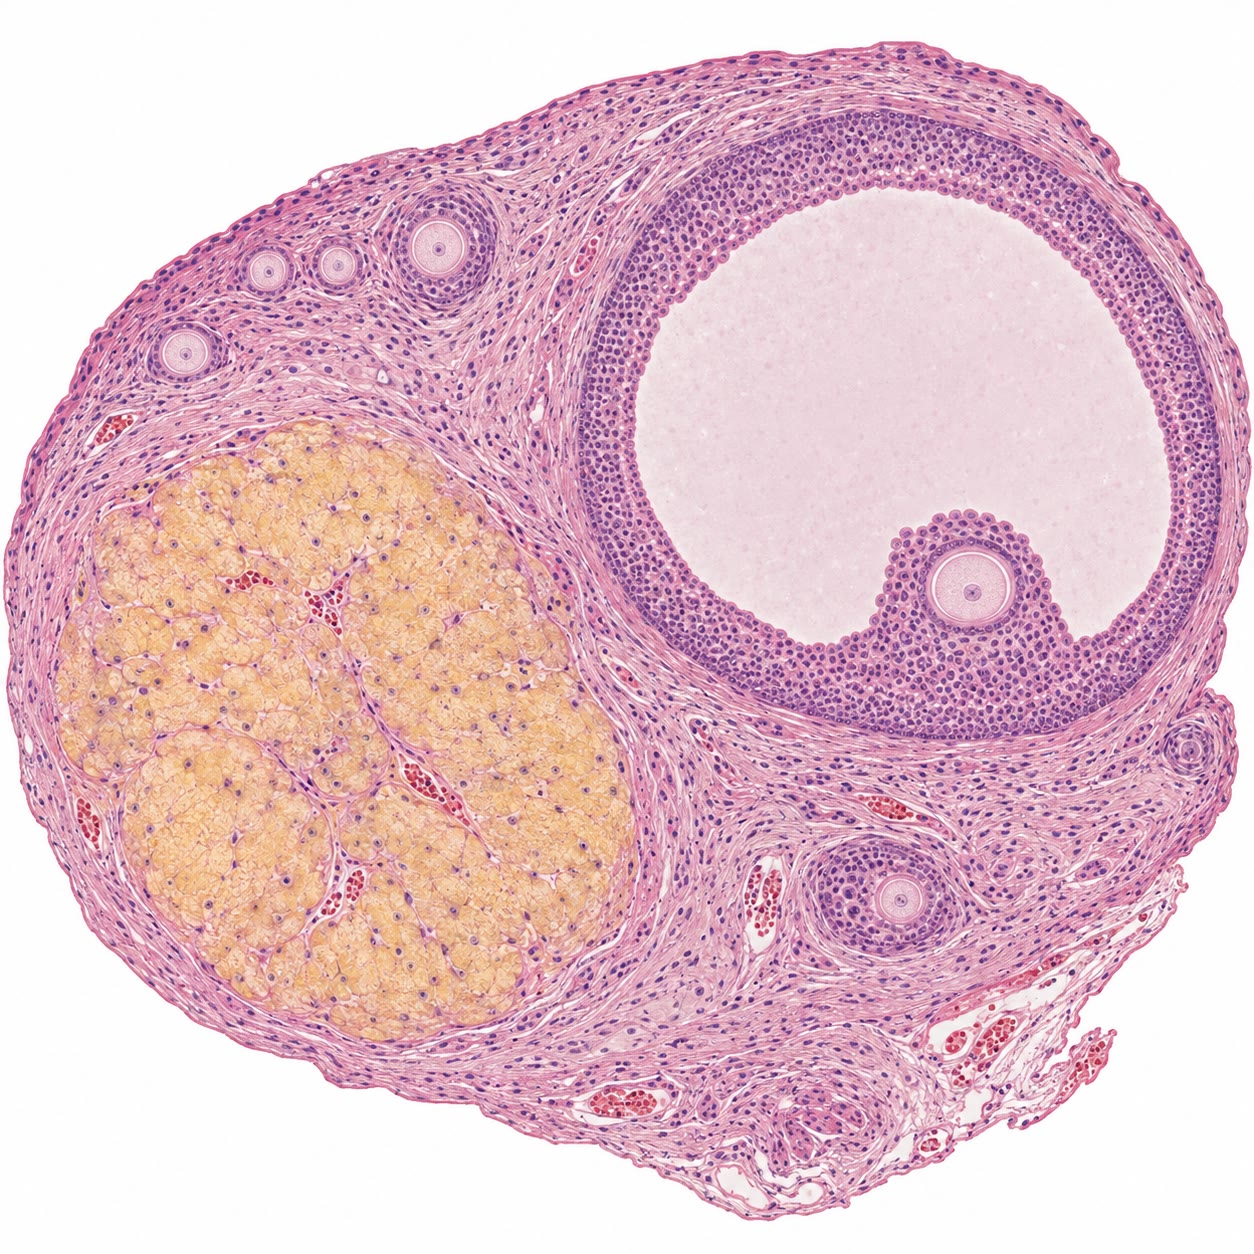
\includegraphics[width=0.46\linewidth]{images/book4/ai/b4-09-ovary-histology.jpg}

{\small Een ovarium in doorsnede: een rijpe \omterm{def:b2:mammal-reproduction:ovary}{follikel} met zijn holte en
oöcyt, kleine primordiale \omterm{def:b2:mammal-reproduction:ovary}{follikels} onder het oppervlak, en een \omterm{def:b2:mammal-reproduction:ovary}{corpus
luteum} uit een vorige cyclus.}
\end{omfigure}

\begin{theorem}[De omslag van negatieve naar positieve terugkoppeling]\label{thm:b2:reproductive-hormones:switch}
\index{positieve terugkoppeling!LH-piek}
Oestradiol in de lage spiegels van de vroege \omterm{def:b2:reproductive-hormones:cycle}{folliculaire fase} remt LH en
FSH; oestradiol boven ongeveer \qty{200}{pg/mL}, gedurende meer dan
ongeveer \qty{36}{h} aangehouden, doet het omgekeerde: het laat de
hypothalamus een stoot GnRH afgeven en de hypofyse daarop antwoorden met
een tienvoudige stijging van LH. Het mechanisme is een omkering van teken,
niet van grootte: een hoge, aanhoudende dosis induceert in de hypofyse een
grote voorraad LH en een verhoogde gevoeligheid voor GnRH, en in de
hypothalamus (via kisspeptineneuronen) een omschakeling van de
GnRH-pulsgenerator naar een piekmodus. De schakelaar zet een graduele
prikkel --- hoeveel oestradiol de \omterm{def:b2:mammal-reproduction:ovary}{follikel} maakt --- om in een
alles-of-niets-gebeurtenis die tot op de dag is getimed, en dat is wat de
\omterm{def:b2:mammal-reproduction:ovary}{ovulatie} vereist; en omdat alleen een grote, rijpe \omterm{def:b2:mammal-reproduction:ovary}{follikel}
\qty{200}{pg/mL} kan volhouden, vuurt de piek alleen als er een eicel klaar
is om vrij te komen. Zodra de \omterm{def:b2:mammal-reproduction:ovary}{ovulatie} heeft plaatsgevonden, herstelt het
progesteron van het \omterm{def:b2:mammal-reproduction:ovary}{corpus luteum} de negatieve terugkoppeling en volgt er
geen tweede piek.
\end{theorem}
\begin{proof}[Bewijsmateriaal]
Bij vrouwen en apen met een onderdrukte as wordt een infuus van oestradiol
dat de plasmaspiegel twee dagen boven \qty{200}{pg/mL} brengt, gevolgd door
een \omterm{def:b2:reproductive-hormones:cycle}{LH-piek}; dezelfde hoeveelheid gedurende één dag, of een lagere spiegel
gedurende drie dagen, niet. Progesteron dat vóór het infuus wordt
gegeven, blokkeert de piek; tegelijk gegeven vervroegt en versterkt het
hem. De drempel in dosis en duur reproduceert de timing van de natuurlijke
piek uit de natuurlijke stijging van oestradiol.
\end{proof}

\section{De cyclus overstemmen}

\begin{proposition}[Zwangerschap, lactatie, menopauze]\label{prop:b2:reproductive-hormones:overrides}
\index{humaan choriongonadotrofine}\index{menopauze}
Een embryo dat zich innestelt, scheidt \emph{hCG} af, een LH-achtig hormoon
dat aan de LH-receptor bindt en het \omterm{def:b2:mammal-reproduction:ovary}{corpus luteum} na zijn veertien dagen in
leven en actief houdt; tegen week tien maakt de \omterm{def:b2:mammal-reproduction:placenta}{placenta} zelf genoeg
progesteron en oestrogenen om de zwangerschap in stand te houden en is het
\omterm{def:b2:mammal-reproduction:ovary}{corpus luteum} overbodig. De hele zwangerschap door houden de hoge
steroïdspiegels LH en FSH op nul: er groeit geen \omterm{def:b2:mammal-reproduction:ovary}{follikel}, er vindt geen
\omterm{def:b2:mammal-reproduction:ovary}{ovulatie} plaats. Na de geboorte verhoogt zogen de prolactine en vertraagt
het de GnRH-pulsen, en blijft de \omterm{def:b2:mammal-reproduction:ovary}{ovulatie} maandenlang onderdrukt. Bij de
\emph{menopauze} is de voorraad \omterm{def:b2:mammal-reproduction:ovary}{follikels} uitgeput: oestradiol en inhibine
dalen, en zonder iets om terug te koppelen stijgen LH en FSH tot tien keer
hun vroegere niveau en blijven daar --- het kenmerk van een klier die niet
meer antwoordt.
\end{proposition}

\begin{proposition}[Anticonceptie en geassisteerde voortplanting]\label{prop:b2:reproductive-hormones:clinic}
\index{anticonceptie!hormonale}\index{in-vitrofertilisatie}
De combinatiepil levert elke dag een synthetisch oestrogeen en een
progestageen: de constante steroïdspiegel houdt FSH en LH laag, er wordt
geen \omterm{def:b2:mammal-reproduction:ovary}{follikel} gerekruteerd, er treedt geen stijging van oestradiol op, en
de piek vuurt nooit; het progestageen maakt ook het slijm van de
baarmoederhals dikker. De stopweek van zeven dagen laat het \omterm{def:b2:reproductive-hormones:cycle}{endometrium}
bloeden; meer dan twee dagen na elkaar pillen vergeten laat FSH ontsnappen,
en er kan een \omterm{def:b2:mammal-reproduction:ovary}{follikel} groeien. Noodanticonceptie stelt de piek met een
hoge dosis progestageen enkele dagen uit. Bij \emph{\omterm{prop:b2:reproductive-hormones:clinic}{in-vitrofertilisatie}}
wordt de as in de omgekeerde richting gestuurd: tien dagen lang dagelijks
FSH doorbreekt de selectie van één dominante \omterm{def:b2:mammal-reproduction:ovary}{follikel} en laat er tien of
meer rijpen; een GnRH-antagonist voorkomt een voortijdige spontane piek;
een injectie met hCG vervangt de piek, en de oöcyten worden 34 tot 36 uur
later geoogst, net voordat ze zouden zijn vrijgekomen; ze worden in het
schaaltje bevrucht en een of twee embryo's worden teruggeplaatst, de rest
wordt ingevroren. Bij mannen onderdrukt toegediend testosteron of een
GnRH-analoog de \omterm{def:b2:mammal-reproduction:testis}{spermatogenese} door LH te onderdrukken --- het principe
van een hormonaal anticonceptiemiddel voor mannen, dat nog niet op de markt
is. Dit alles is de as uit de eerste paragraaf, achterstevoren gelezen.
\end{proposition}

\section{Opgaven}

\begin{exercise}[$\star$]\label{exo:b2:reproductive-hormones:1}
Teken de as voor de man: de drie niveaus, de vier hormonen, de twee
terugkoppelingslussen, en de cellen waarop elk hormoon inwerkt.
\end{exercise}

\begin{exercise}[$\star$]\label{exo:b2:reproductive-hormones:2}
Geef de fasen van de ovariële en de uteriene cyclus met hun dagen en het
hormoon dat in elke fase overheerst.
\end{exercise}

\begin{exercise}[$\star$]\label{exo:b2:reproductive-hormones:3}
Leg uit hoe de combinatiepil de \omterm{def:b2:mammal-reproduction:ovary}{ovulatie} verhindert, en waarom er in de
stopweek een bloeding optreedt.
\end{exercise}

\begin{exercise}[$\star$]\label{exo:b2:reproductive-hormones:4}
Wat gebeurt er met LH, FSH en de secundaire geslachtskenmerken van een
gecastreerde volwassen man? Welke daarvan keert ingespoten testosteron om,
en welke niet?
\end{exercise}

\begin{exercise}[$\star\star$]\label{exo:b2:reproductive-hormones:5}
GnRH-pulsen komen om de \qty{90}{min} in de \omterm{def:b2:reproductive-hormones:cycle}{folliculaire fase} en om de
\qty{4}{h} in de \omterm{def:b2:reproductive-hormones:cycle}{luteale fase}. Hoeveel pulsen per dag zijn dat in elke fase?
De hypofyse bevoordeelt LH bij snelle pulsen en FSH bij trage: welk
gonadotrofine zou als eerste moeten stijgen wanneer het \omterm{def:b2:mammal-reproduction:ovary}{corpus luteum}
sterft, en waarom is dat het juiste?
\end{exercise}

\begin{exercise}[$\star\star$]\label{exo:b2:reproductive-hormones:6}
Zet \qty{200}{pg/mL} oestradiol (molaire massa
\qty{272}{g/mol}) om in \unit{pmol/L}, en \qty{15}{ng/mL}
progesteron (\qty{314}{g/mol}) in \unit{nmol/L}. Hoeveel
moleculen oestradiol bevat één microliter plasma bij de drempel van de
piek?
\end{exercise}

\begin{exercise}[$\star\star$]\label{exo:b2:reproductive-hormones:7}
De cycli van een vrouw duren 35 dagen. Op welke dag ovuleert ze, gegeven
dat de \omterm{def:b2:reproductive-hormones:cycle}{luteale fase} vastligt, en welke dagen zijn vruchtbaar als
zaadcellen drie dagen overleven en de eicel één? Waarom faalt de
kalendermethode bij onregelmatige cycli?
\end{exercise}

\begin{exercise}[$\star\star$]\label{exo:b2:reproductive-hormones:8}
Een embryo nestelt zich in op dag 21 van een cyclus van 28 dagen en zijn
hCG verdubbelt, beginnend bij \qty{1}{IU/L}, om de twee dagen. Het \omterm{def:b2:mammal-reproduction:ovary}{corpus
luteum} heeft tegen dag 26 enkele IU/L hCG nodig om te overleven. Is het
embryo op tijd? Wat zou er gebeuren als de \omterm{def:b2:mammal-reproduction:implantation}{innesteling} tot dag 25 werd
uitgesteld?
\end{exercise}

\begin{exercise}[$\star\star$]\label{exo:b2:reproductive-hormones:9}
Zeg wat het experiment van Knobil aantoonde en wat het uitsloot, en
voorspel het effect van een maand lang toedienen van een langwerkende
GnRH-agonist aan een vrouw: op LH, op oestradiol, op het \omterm{def:b2:reproductive-hormones:cycle}{endometrium}.
\end{exercise}

\begin{exercise}[$\star\star\star$]\label{exo:b2:reproductive-hormones:10}
Neem in het receptormodel $s = 100$ receptoren per uur, $d =
\qty{0.5}{h^{-1}}$ en $iH = \qty{6}{h^{-1}}$ zolang er hormoon aanwezig is.
Bereken het stationaire aantal receptoren zonder hormoon en met continu
hormoon. Bereken bij een puls van twee minuten per uur het aantal dat per
puls verloren gaat en de fractie van het tekort die vóór de volgende puls
is hersteld, en leid af rond welk niveau de voorraad zich instelt.
\end{exercise}

\begin{exercise}[$\star\star\star$]\label{exo:b2:reproductive-hormones:11}
Een vrouw na de menopauze heeft LH en FSH van tien keer het niveau van een
jonge vrouw en een zeer laag oestradiol; een vrouw met een hypofysetumor
die prolactine afscheidt, heeft een laag LH, een laag oestradiol en geen
cycli; een vrouw met een granulosaceltumor heeft een hoog oestradiol, een
laag LH en geen cycli. Verklaar elk profiel vanuit de as.
\end{exercise}

\begin{exercise}[$\star\star\star$]\label{exo:b2:reproductive-hormones:12}
``Hetzelfde hormoon remt en zet vervolgens de \omterm{def:b2:reproductive-hormones:cycle}{LH-piek} in gang.'' Leg uit
hoe oestradiol beide effecten kan hebben, waarom de \omterm{def:b2:mammal-reproduction:ovary}{ovulatie} een
schakelaar nodig heeft in plaats van een draaiknop, en wat er met een
draaiknop mis zou gaan.
\end{exercise}

\section{Vraagstuk: een gemeten cyclus}

\begin{problem}[{Weekendvraagstuk --- dagelijkse hormoonmetingen van één
cyclus worden gelezen op hun fasen, de ovulatiedag en het vruchtbare
venster; de drempel van de piek, de klok van het corpus luteum en de
redding door hCG worden berekend; het receptormodel verklaart Knobil; en
de as wordt in de kliniek achterstevoren gestuurd, met als besluit de
ovulatiedag, de lengte van de luteale fase, het vruchtbare venster en de
drempel van de piek}]
\label{pb:b2:reproductive-hormones:1}
Op geselecteerde dagen van de cyclus van een vrouw werd bloed afgenomen:

\begin{center}
\small
\begin{tabular}{lcccccccccc}
\hline
dag & 1 & 5 & 8 & 11 & 12 & 13 & 14 & 15 & 21 & 27 \\
\hline
oestradiol (\unit{pg/mL}) & 40 & 60 & 110 & 210 & 260 & 310 & 220 & 150 & 160 & 50 \\
LH (\unit{IU/L}) & 5 & 5 & 6 & 7 & 8 & 20 & 65 & 15 & 4 & 4 \\
progesteron (\unit{ng/mL}) & 0.5 & 0.5 & 0.6 & 0.7 & 0.8 & 1.0 & 1.5 & 3 & 16 & 2 \\
temperatuur (\unit{\celsius}) & 36.4 & 36.4 & 36.4 & 36.4 & 36.4 & 36.4 & 36.4 & 36.5 & 36.8 & 36.7 \\
\hline
\end{tabular}
\end{center}

De menstruatie begon op dag 1 en opnieuw op dag 29.

\medskip
\noindent\textbf{Deel I --- De cyclus lezen.}
\begin{enumerate}
  \item Wijs in de tabel de folliculaire en de \omterm{def:b2:reproductive-hormones:cycle}{luteale fase} aan, met het
        hormoon dat elke fase kenmerkt.
  \item Op welke dag piekte de \omterm{def:b2:reproductive-hormones:cycle}{LH-piek}? Wanneer vond de \omterm{def:b2:mammal-reproduction:ovary}{ovulatie} plaats?
  \item Hoelang duurde de \omterm{def:b2:reproductive-hormones:cycle}{luteale fase}? Klopt dat met de levensduur van het
        \omterm{def:b2:mammal-reproduction:ovary}{corpus luteum}?
  \item Verklaar de temperatuurverschuiving en waarom die de \omterm{def:b2:mammal-reproduction:ovary}{ovulatie} wel
        bevestigt maar niet kan voorspellen.
  \item Op welke dagen lag oestradiol boven \qty{200}{pg/mL}? Breng de duur
        in verband met de piek.
  \item Geef het vruchtbare venster van deze cyclus (zaadcellen drie dagen,
        eicel één dag).
\end{enumerate}

\medskip
\noindent\textbf{Deel II --- Getallen.}
\begin{enumerate}[resume]
  \item Zet het oestradiol van dag 13 om in \unit{pmol/L}, en het
        progesteron van dag 21 in \unit{nmol/L}.
  \item Met welke factor steeg LH van dag 12 tot dag 14? Waarom daalt het
        daarna zo snel (de halveringstijd van LH is ongeveer
        \qty{1}{h})?
  \item Als de volgende cyclus van deze vrouw een \omterm{def:b2:reproductive-hormones:cycle}{folliculaire fase} van 21
        dagen had, op welke dag zou ze dan ovuleren en hoe lang zou de
        cyclus duren?
  \item Een embryo nestelt zich 7 dagen na de \omterm{def:b2:mammal-reproduction:ovary}{ovulatie} in. Op welke dag van
        deze cyclus zou hCG verschijnen, en welk niveau zou het, verdubbelend
        om de twee dagen vanaf \qty{1}{IU/L}, tegen dag 27 bereiken?
  \item Leg uit waarom het progesteron van \qty{2}{ng/mL} op dag 27 aantoont
        dat er geen embryo is ingenesteld.
  \item Wat zouden de waarden van progesteron en oestradiol op dag 27
        geweest zijn als dat wel zo was?
\end{enumerate}

\medskip
\noindent\textbf{Deel III --- Terugkoppeling en pulsen.}
\begin{enumerate}[resume]
  \item Leg met de tekens van de terugkoppeling uit waarom FSH aan het begin
        van de cyclus het hoogst is en waarom meestal maar één \omterm{def:b2:mammal-reproduction:ovary}{follikel}
        overleeft.
  \item Bereken in het receptormodel met $s = 100$ per uur, $d =
        \qty{0.5}{h^{-1}}$, $iH = \qty{6}{h^{-1}}$ de waarde $R^*$
        zonder hormoon en onder continu hormoon.
  \item Een puls duurt \qty{2}{min}. Hoeveel receptoren verwijdert één puls,
        uitgaande van de ongestimuleerde
        $R^*$ (gebruik de lineaire benadering $iHR\,\Delta t$)? Welke fractie
        van het tekort wordt hersteld in het uur vóór de volgende puls
        (tijdconstante $1/d$), en rond welk niveau stelt de voorraad zich
        in?
  \item Gebruik deze getallen om het resultaat van Knobil te verklaren.
  \item Een man krijgt voor prostaatkanker continu een GnRH-agonist.
        Voorspel zijn LH en testosteron na één dag en na één maand, en leg
        het verschil uit.
  \item De granulosacellen van een vrouw maken geen inhibine. Voorspel haar
        FSH en LH, en het gevolg voor de rekrutering van \omterm{def:b2:mammal-reproduction:ovary}{follikels}.
\end{enumerate}

\medskip
\noindent\textbf{Deel IV --- De kliniek.}
\begin{enumerate}[resume]
  \item Voor \omterm{prop:b2:reproductive-hormones:clinic}{in-vitrofertilisatie} krijgt deze vrouw vanaf dag 2 dagelijks
        FSH. Leg uit waarom er tien \omterm{def:b2:mammal-reproduction:ovary}{follikels} rijpen in plaats van één.
  \item Waarom wordt vanaf dag 6 een GnRH-antagonist toegevoegd, en wat zou
        er zonder gebeuren?
  \item hCG wordt ingespoten wanneer de \omterm{def:b2:mammal-reproduction:ovary}{follikels} rijp zijn; de oöcyten
        worden 35 uur later geoogst. Verantwoord deze timing aan de hand van
        de tabel.
  \item Er worden tien oöcyten geoogst; \qty{70}{\%} wordt bevrucht,
        \qty{40}{\%} van de embryo's bereikt het blastocystestadium, en elke
        teruggeplaatste \omterm{def:b2:mammal-reproduction:implantation}{blastocyste} nestelt zich in met kans $0.35$.
        Verwacht aantal \omterm{def:b2:mammal-reproduction:implantation}{blastocysten}? Kans op minstens één zwangerschap als
        er twee worden teruggeplaatst?
  \item Leg uit waarom de combinatiepil, door deze vrouw genomen, een tabel
        zou hebben opgeleverd zonder \omterm{def:b2:reproductive-hormones:cycle}{LH-piek} en zonder stijging van het
        progesteron.
  \item Een anticonceptiemiddel voor mannen op basis van een
        GnRH-antagonist zou ook het testosteron wegnemen. Wat moet er samen
        mee worden gegeven, en waarom herstelt dat de zaadproductie niet?
  \item Formuleer het resultaat: ovulatiedag, lengte van de \omterm{def:b2:reproductive-hormones:cycle}{luteale fase},
        vruchtbaar venster, en de drempel en de duur van oestradiol die de
        piek in gang zetten.
\end{enumerate}
\end{problem}
